In this section we talk about related work and a description of lazart tool.
\subsection{Fault injection}
Fault injection is an old, well-studied attack models in security and cryptology that can be created at hardware or software level\cite{liu2025}.
While multiple methods exist multiple methods to simulate fault injection, one approach involves hardware-based techniques, such as \cite{Richter-Brockmann2021,Arribas2020}. 
Another method to simulate fault injection is using software tools \cite{Lazart2015,Riviere2014}. 
One sush software tool is called Lazart \cite{Lazart2015}.
A countermeasure benchmark, developed using the Lazart tool by several researchers, is FISSC \cite{dureuil2016}.  

While a few studies have been conducted on countermeasures in Rust \cite{21Kim2026ICCE,22Sini2025DATE} ,there is little research that has been conducted on comparing the results between C and Rust for countermeasures.

Furthermore, little research has been done on the effectiveness of the protecting of the countermesure from compiler optimisations.
We addressed this gap by highlighting the work of Sébastien Michelland \cite{23miche2025}.

\subsection{Lazart tools}
\label{subsec:Lazart}
\begin{figure*}
    \centering
    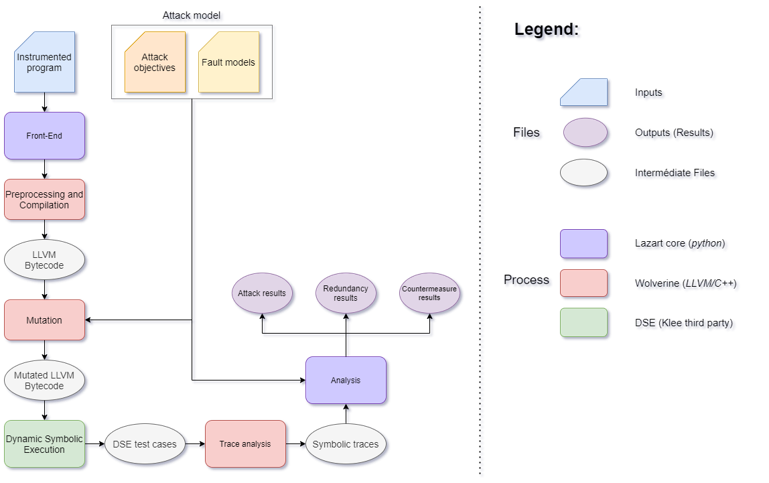
\includegraphics{image/lazart-arch.png}
    \caption{Lazart tool arkitecture}
    \label{figure_0:Lazart}
\end{figure*}

Lazart \cite{Lazart2015} is a high level fault injection tool.
Has been develop by Verimag since 2015.
It allows to identifying vulnerable paths in code and can be used to evaluate the accuracy of countermeasures against a given fault model and a security property.
Unlike other similar tools, Lazart is one of the few that are capable of performing multi-fault attacks.
Lazart is able to analyse C or C++ code by compiling it using the Clang compiler.
They use one of the features of Clang to generate LLVM bitecode (which is Intermediate code).\\
LLVM is a middle component of the compiler and is designed for compile-time, link-time and run-time optimisation.
The LLVM framework is run by Clang after the frontend pipeline is completed.

Lazart is composed of five step:
\begin{enumerate}[noitemsep,leftmargin=0em,wide]
\item Preprocessing and compilation of the input code.
\item Mutation of the code with Wolverine.
\item Dynamic-Symbolic Execution with KLEE \cite{24Cadar2008KLEEUA,25kleeseKLEE}.
\item Trace parsing from KLEE's outputs.
\item Analysis.
\end{enumerate}

Lazart can support 4 fault models:
\begin{itemize}[noitemsep,leftmargin=0em,wide]
    \item Test inversion (modification of the evaluation of a branch condition);
    \item data mutation (modification of the loaded values);
    \item instruction skip;
    \item Call another function (function switch);
\end{itemize}

\todo[inline]{under new section}

\subsection{Rust Language}
Rust is a general-purpose programming language which emphasizes performance, type safety, concurrency, and memory safety.
Rust has is first version released in 2006.
One of features of rust is the way hwo it handle the memory safety and concurrency of a program.
Unlike other language who use a garbage colector, Rust use a "barrow checker" that track the life spand of a variable as there owner.
And deal with data races. 

\subsubsection{Why using Rust ?}
We give several reason of using rust: 
\begin{itemize}
    \item Rust use the same LLVM as clang does in C/C++. So it make Rust compatible with lazart.
    \item Rust is a recent,still updated programming language.
    \item Rust is used for embeded system.
\end{itemize}

\subsubsection{The usage of no\_std}
One point that need to be explain on this reporte is the flag no\_std.
Using no\_std attribute stops the compiler from linking std into the crate, and only links core.
It limit :
\begin{itemize}
    \item Heap allocation.
    \item File I/O, threading, and networking.
    \item Many common traits and types (e.g., std::io::Error).
\end{itemize}

\todo[inline]{below new section}